\section{Vector Extensions}

As it was previously discussed, enhancing data load and store operations contributes to the improvement of the system's memory access latency and overall performance. However, individual computations on this data still occur sequentially. This is where vector extensions prove beneficial. Vector extensions employ Single Instruction, Multiple Data (SIMD) instructions across a vector of data in a single execution step, enabling increased system throughput.


\subsection{ARM Scalable Vector Extention}
\label{label:arm-sve}

The ARM approach to a vector-length-agnostic programming model was the definition of ARM SVE \cite{arm-paper}. SVE brings a new architectural state with the inclusion of:
\begin{itemize}
    \item 32 new scalable vector registers, \textit{Z0 to Z31}, with a total width ranging from 128 to 2,048 bits depending on the implementation;
    \item 32 128-bit wide Advance SIMD registers, \textit{V0 to V31}, allowing for 64-, 32-, 16- and 8-bit scalable containers
    \item 16 scalable predicate registers \textit{P0 to P15} and a set of control registers \textit{ZCR\_EL1 to ZCR\_EL3}.
\end{itemize}


\subsubsection{Predication}
The ARM SVE solution allows programmers to think at a higher level of abstraction regarding vector length. This is possible through predicate registers that dynamically modify the vector length during execution. This technique allows the computation of only those lanes that matter, as opposed to the usual SIMD strategy of computing the whole vector and discarding unwanted values through masking.

\begin{figure}[H]
	\begin{center}
 		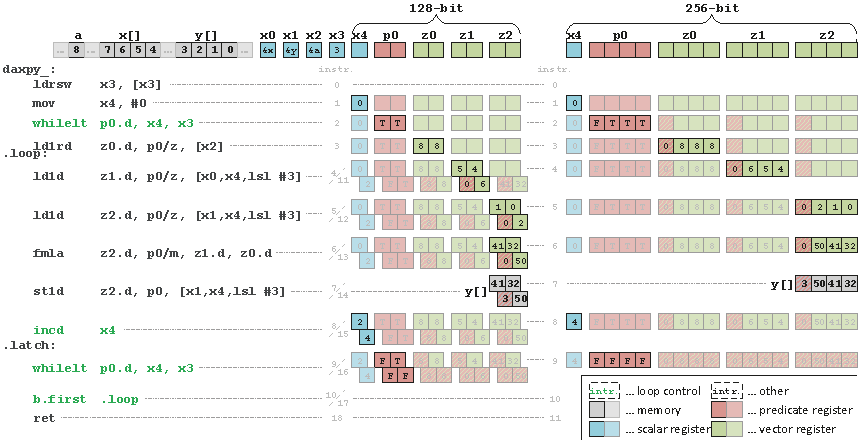
\includegraphics[width=0.77\linewidth]{images/predicator-example.pdf}
 		\caption{Cycle by cycle example of daxpy with n = 3 and hardware vector lengths of 128- and 256-bit - Figure from \cite{arm-paper}}
 		\label{fig:arm-sve-assembly}
	\end{center} 
\end{figure}

Figure \ref{fig:arm-sve-assembly} illustrates a step-by-step example of a Daxpy program for a vector length of 128 and 256 bits. The use of a predicate variable is demonstrated in the 128-bit configuration, with both its values set to true on the first comparison, utilizing the full dimension of the vector. This state of the predicate signifies that the load and computation of values occur in both positions of the variables \textit{z0, z1, z2}. After the loop iteration,  the variable tracking the number of processed elements is incremented (in this case, by the total number of float elements in the vector), and compared with the total number of values to be processed. From this comparison, another predicate is generated, and, since two elements have been processed and the total is three, the new predicate indicates the execution of instructions over only a single entry of \textit{z0, z1, z2} in the next iteration.

Something similar happens in the 256-bit vector configuration. However, the initial comparison generates a predicate with the last position being false. This means the vector won't be utilized in full, and the next predicated instructions to execute should only compute three values.

SVE also includes in its extended instruction set a family of \textit{while} instructions that operate by populating a new predicate through the use of a scalar counter. The value of this stride can be incremented not only by the value of the total number of elements in the system vector but also through more complex increment functions like incrementing by the number of active lanes, or the largest multiple of a data element on a vector, allowing for a powerful data access and manipulation. 

Due to this nature of vector-length-agnostic programming, situations that require vector initialization can become more difficult. To address this complexity, the SVE extension incorporates a set of instructions capable of dynamically generating vector initialization during runtime. This dynamic approach is particularly useful as it adapts to pattern initializations, allowing for flexibility and efficiency in vector initialization processes.

Some examples of specific vector initialization are as follows:
\begin{itemize}
    \item Initializing a vector with a set of indexes that start on 1 and increment by 4 can be achieved using \textit{INDEX Zd.S, \#1, \#4} resulting in \textbf{Zd = [1, 5, 9, 13, 17, 21, 25, 29]} for a vector size of 8 elements.
    \item Initializing a predicate vector that is supposed to contain as many triples of the true value as will fit in the vector:\textit{PTRUE Pd.S, MUL3} will result in  \textbf{Pd = [(T,T,T), (T,T,T), F, F]} for a vector size of 8 elements.
\end{itemize}

\subsubsection{Horizontal Reductions}

Another implemented feature in ARM SVE is the ability to do operations across lanes of a vector, essentially taking an operation and applying it to every element of the vector, for example, a sum, a bitwise-and, etc. 

Designing a program with these intrinsics in mind allows for better performance. Fig. \ref{fig:horizontal-reductions} shows the compiled code of a sum of a multiplication of two vectors with and without intrinsics. Both compiled versions of code execute at the beginning of each loop iteration the load of the values of $a$ and $b$ (green instructions), the differences occur on the computation part of each iteration. In the ARM SVE version without intrinsics (Fig. \ref{fig:horizontal-reductions}.C), the loaded vectors are multiplied, and the result is stored in a vector (purple instruction) following that instruction, a sum of values occurs by adding each entry of the vector to the register $d0$ this leads to the increase of the number of operations that occur per iteration.

In the ARM SVE version with intrinsics (Fig. \ref{fig:horizontal-reductions}.D), a horizontal reduction instruction is used at the end, meaning that during the loop iterations, it is more advantageous to multiply the vectors and add the result to third temporary vector (yellow instruction - fmla). The advantage comes from the fact that the instruction can happen across the vector entries simultaneously, resulting in a lighter computational pressure when compared with the previously compiled code. To achieve the same final result at the end of the execution, the horizontal reduction sums the entries of the final resulting vector.

Even though both Fig. \ref{fig:horizontal-reductions}.C and \ref{fig:horizontal-reductions}.D appear to have similarly sized loops, the executed instructions differ a lot in terms of execution time, with the ARM SVE version with intrinsic reaching the final result faster.

\begin{figure}[H]
	\begin{center}
 		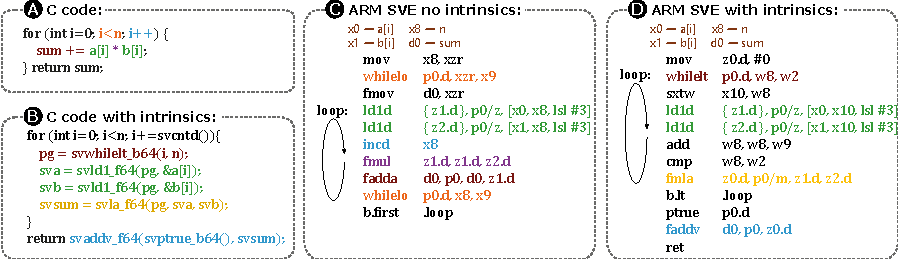
\includegraphics[width=\linewidth]{images/horizontal-reductions.pdf}
 		\caption{Comparison of assembly code between ARM SVE without and with horizontal intrinsics}
 		\label{fig:horizontal-reductions}
	\end{center} 
\end{figure}

\subsubsection{Handling unknown data vector size}


In earlier instances of ARM SVE examples, predicates have consistently played a crucial role in the loading, storing, and manipulation of data. Nevertheless, scenarios may arise where determining the size of the vector becomes impractical before the data load. 

One approach in such situations could be to load as much data as can be fitted into a vector. However, this approach introduces the risk of loading invalid or protected values from memory, potentially triggering a fault.

To avoid the aforementioned problem, speculative vectorization can be utilized. SVE incorporates a distinctive predicate, the First Fault Register (FFR), generated when employing a memory-probing instruction. This instruction essentially examines the memory entries, starting at a base address, and return a predicate that indicates the regions in memory corresponding to the desired data.


This feature facilitates the vectorization of uncounted loops with break conditions without the need for explicit size specification. Figure \ref{fig:ffr-example} illustrates the utilization of a memory-probing instruction, the \textit{LDFF1D}, within an uncounted loop, and will be explained in the following paragraphs.


During the initial iteration of the probing instruction, all memory entries are examined, as the P1 predicate is initialized as entirely true. The resulting Forwarding Flag Register (FFR) signifies that data on the initial 2 entries of the memory can be accurately loaded, given the presence of correct data.

In the subsequent iteration, the P1 predicate register is modified to turn each entry false where the FFR indicates true. In this specific example, this adjustment ensures that the next probing instruction will disregard the first two entries of the vector. The probing instruction then generates a new FFR, and as its first entry is false, it triggers an operating system trap, indicating that the end of the vector has been reached.



\begin{figure}[H]
	\begin{center}
 		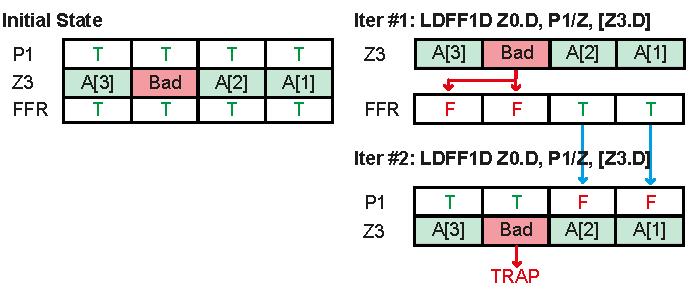
\includegraphics[width=0.77\linewidth]{images/ffr-example final.pdf}
 		\caption{Simplified example of loop iteration and vector partition with FFR}
 		\label{fig:ffr-example}
	\end{center} 
\end{figure}

Nevertheless, while this feature effectively addresses the challenge posed by an unknown data size, it introduces a potential downside. The increase in the number of instructions within the loop may contribute to heightened pressure on the processor pipeline. This, in turn, could impact the overall efficiency of the vectorization process. Balancing the advantages of dynamic size handling with the potential impact on pipeline performance becomes a crucial consideration in optimizing the execution of SVE instructions.

\subsubsection{Result Analysis}

 The authors of ARM SVE \cite{arm-paper} conducted a series of workloads in 4 different configurations of the same generic medium-sized out-of-order microprocessor, one without the implementation of SVE, and three implementations with SVE and where the vector size was changed to 128-, 256- or 512-bit vector length.
The overall results of the SVE implementations showed significant speedups, with workloads achieving 3x, 5x and 7.5 gains for the SVE 128-bit, SVE 256-bit, and SVE 512-bit implementation, respectively, when compared with the non-SVE implementation. Some workload tests presented no speedup due to the nature of the test since they do not benefit from vectorization, so performance was very similar between the four configurations.



\subsection{RISC-V Vector Extention (RVV)}
\label{label:rvv}

Just like the ARM Scalable Vector Extension (SVE), the \acrfull{RVV} adopts an \acrfull{ISA} that centers around a vector-length-agnostic programming model. \acrshort{RVV} operations distinguish themselves solely based on vector-vector and vector-scalar distinctions, considering signed and unsigned types, without specifying element lengths. Consequently, the element length becomes a dynamic parameter in this context. Moreover, \acrshort{RVV} allows the utilization of only a segment of a vector register or even a combination of multiple vector registers, introducing the necessity for dynamic parameters in such scenarios.


The \acrlong{RVV} introduces a collection of 32 variable-length vector registers and 7 context and status registers (CSRs). These additional CSRs are integrated into the base scalar RISC-V ISA and serve the purpose of storing the vector configuration of the currently executing application. Among the configurations maintained by these CSRs are the vector length, data type, and the starting position of the vector.

\subsubsection{Operations and Execution}

The manipulation of vectors is facilitated through the implementation of a new set of instructions introduced with the \acrshort{RVV} extension. This extension supports typical arithmetic operations for both fixed and floating-point data, along with reduction operations such as sum, max, and min. Additionally, certain instructions can be customized through the use of masking, allowing the disabling or enabling of specific vector elements during processing.

In Fig. \ref{fig:uve-comparison}, an example of a simple saxpy application compiled with the RVV extension is illustrated. Throughout the loop iteration, vector registers used to store data and vector-specific instructions to manipulate the vectors. At the beginning of the loop, an instruction ($vsertvli$) is utilized to define the characteristics of the vector, including its length and data type.






\subsection{Unlimited Vector Extention with Data Streaming Support}
\label{label:uve}

%Unlimited Vector Extention is a novelty solution that aims to surpass the existing problems of current state-of-the-art solutions of scalable vector extensions through the use of a data streaming engine, combining streaming and SIMD processing, which allows the exploitation of data parallelism.


%The proposed ISA tries to reduce latencies associated with loop control, memory access indexing, and memory access by using new instructions that allow a pre-configuration of the stream and the memory access patterns. 
%This anticipation of the access control allows for accurate and fast prefetching even with multidimensional arrays or indirect memory accesses. 


The \acrfull{UVE} \cite{uve-paper} represents a novel solution designed to combine faster data access with increased system throughput. Achieving this objective involves the incorporation of a data streaming engine that seamlessly integrates streaming and SIMD processing, thereby enabling the effective utilization of data parallelism.

The envisioned \acrshort{ISA} strives to mitigate latencies commonly associated with loop control, memory access indexing, and memory access. This is achieved by introducing novel instructions that facilitate the pre-configuration of the data stream and memory access patterns. The innovative feature of reconfiguration of access control enables precise and expedited prefetching, even when dealing with multidimensional arrays or indirect memory accesses.


\subsubsection{UVE Features}

\begin{figure}[H]
    \centering
    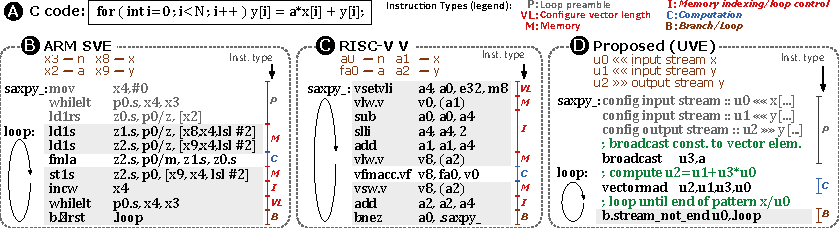
\includegraphics[width=\linewidth]{images/UVE-Comparison.pdf}
    \caption{Assembly code comparison between ARM SVE, RVV, and UVE - Figure from \cite{uve-paper}}
    \label{fig:uve-comparison}
\end{figure}

The main difference of this solution from other recently developed SIMD solutions (ARM SVE and RISC-V Vector extension (RVV)) comes from features like:
\begin{itemize}
\item[]  \Tbullet{F1}{Decoupled Memory Access} The ability to decouple the memory accesses from the computation part by streaming the data directly to the register, allowing the occurrence of loads/stores in parallel with the data manipulation, thus reducing the memory access latency.


\item[]  \Tbullet{F2}{Indexing-free Loops} By describing the load/store patterns in advance, it allows minimizing the number of instructions related to memory indexing, reducing the pressure on the processor pipeline (see Fig.\ref{fig:uve-comparison}.D). 



\item[]  \Tbullet{F3}{Simplified Vectorization} The use of memory access pattern descriptors allows the Streaming Engine to anticipate all non-coalesced accesses as linear patterns and deliver them to the processing unit. This leads to a simplified vectorization since memory is always aligned from the execution pipeline point of view - see Fig. \ref{fig:uve-mem-access}. 


\item[]  \Tbullet{F4}{Implicit Load/Store} Since the streams are described in the loop preamble, the indexing instructions can be removed, meaning that all explicit loads and stores are associated with active streams and different vector registers.
\end{itemize}

Besides the mentioned features, UVE is also register-size agnostic, similar to SVE and RVV. However, in UVE, there is no need for size control instruction since the Streaming Engine automatically disables all vector elements that fall out of bounds, making the loops simpler with a minimal set of control functions.


\begin{figure}[H]
	\begin{center}
 		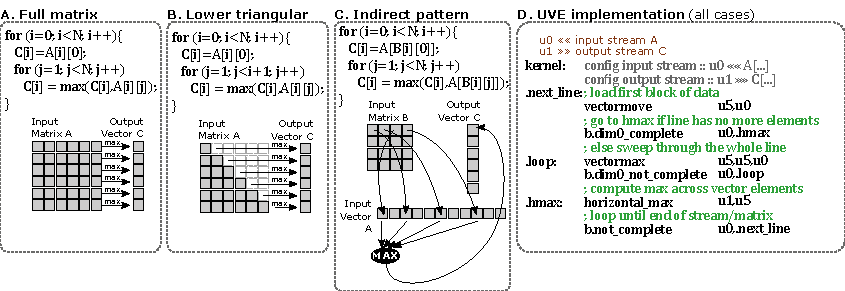
\includegraphics[width=\linewidth]{images/UVE-pseudo-code.pdf}
 		\caption{UVE pseudo-code implementation for the computation of the maximum
across the rows on three possible matrices: (A) full matrix, (B) lower triangular
matrix, and (C) full matrix with pointers to an array - Figure adapted from \cite{uve-paper}}
 		\label{fig:uve-mem-access}
	\end{center} 
\end{figure}


\subsubsection{Microarchiteture Extension}

In order to decouple the memory accesses the \acrshort{UVE} implementation proposed by, Domingos \textit{et al.} \cite{uve-paper} assumed the incorporation of a streaming engine in the microarchitecture of a CPU core. Adding such a feature requires the modification of other preexisting components, like the instruction decoder (to support SIMD operations as well as the streams configuration, control, and manipulation instructions)  modifying the reorder buffer to enable the renaming of vector registers and streams, allowing for speculative stream configuration, and lastly, add a new execution unit on the execution stage to process all the stream manipulating instructions. The proposed changes and their placement can be seen in Fig. \ref{fig:uve-arch}.

\begin{figure}[H]
	\begin{center}
 		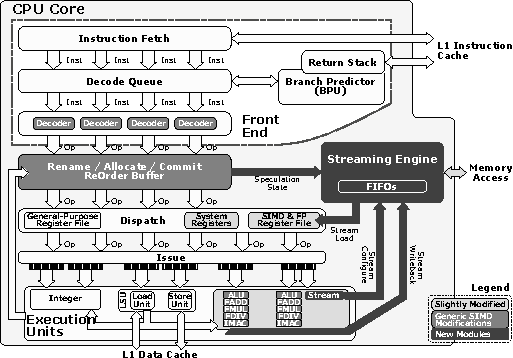
\includegraphics[width=0.67\linewidth]{images/UVE-arch.pdf}
 		\caption{Modifications overview for UVE support}
 		\label{fig:uve-arch}
	\end{center} 
\end{figure}

The implemented streaming engine has the responsibility of managing all the input and output streams. Its inner structure is depicted in Figure \ref{fig:uve-engine} and is composed of 4 main modules: the \acrfull{SCROB} (unit corresponding to the sorting queue and validation on the left of Figure \ref{fig:uve-engine}), a stream table, a stream scheduler and address generator, and a set of load/store FIFO queues.

\begin{figure}[H]
	\begin{center}
 		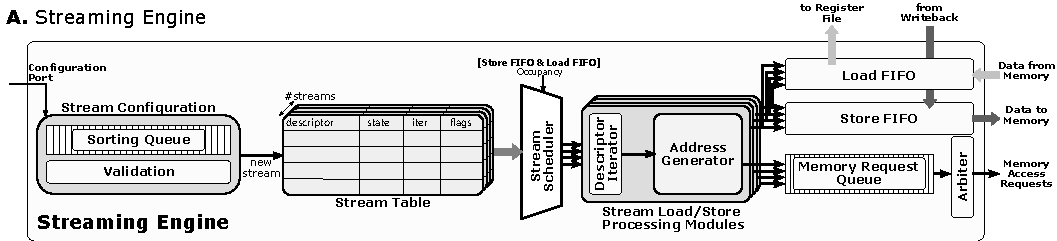
\includegraphics[width=0.97\linewidth]{images/uve-engine.pdf}
 		\caption{Streaming engine structure}
 		\label{fig:uve-engine}
	\end{center} 
\end{figure}


The Stream processing starts with the configuration of the streams. Whenever a configuration instruction reaches the rename stage of the pipeline, it is moved to the first unit of the streaming engine, the stream configuration queue, where it will wait until all operands of the configuration descriptor are available. This approach of using a dedicated buffer unit is used since complex access patterns might require multiple instruction and holding such instructions on the pipeline commit buffer would prevent the speculative configuration of streams, impacting performance. Following the validation of the configuration, the configured stream is moved to the stream table, allowing the stream scheduler to start processing the stream by either pre-loading data for inputs (storing these requests in the memory requests queue and data on the Load FIFO) or calculating addresses for outputs (storing the generated addresses into the Store FIFO). 

The iteration of the chosen streams occurs at each clock cycle and is decided through prioritization of lower FIFO occupancy, by the stream scheduler. Each stream processing model receives a stream and processes it according to their descriptor configuration values, iterating a single dimension and corresponding modifier at a time (this allows for a lower hardware complexity and size).  On each iteration, an update is made to the stream table, keeping the table entries synchronized with the stage of each processed stream. 


\subsubsection{Data Streaming Descriptors}

As mentioned in the previous section, the configuration of streams is encoded in a descriptor-based representation. These descriptors provide the necessary values/parameters utilized on the proposed address modeling equation, defined by Eq. \ref{eq:mem_model}. 

\begin{equation}
    y(X) = y_{\text{base}} + \sum_{k=0}^{\text{dim}_y} x_k \times S_k
    \quad \text{with } X = \{x_0, \ldots, x_{\text{dim}_y}\} \text{ and } x_k \in [O_k, E_k+O_k]
    \label{eq:mem_model}
\end{equation}

Stream descriptors can be classified into two types: \textit{Base Stream Descriptor} and \textit{Descriptor Modifiers}.

\textbf{Base Stream Descriptors} define a uni-dimensional access pattern. It is represented by three-parameters $\{O, E, S\}$ corresponding to the offset $(O_k)$, the size $(E_k)$ and the stride $(S_k)$. These patterns configure the base address of the memory access through the offset value $(O_k)$, the total size of the stream to be loaded/stored with $(E_k)$, and the value of the interleaving space between memory accesses with $(S_k)$. Examples of simple patterns supported by descriptors of this type can be seen in Figs. \ref{fig:stream-descriptors}.B1, B2 and B3.

\textbf{Static Descriptors Modifiers} are descriptors that can be used in conjunction with parameters of Base Stream Descriptors to modify the access pattern, allowing for loop-conditioned accesses, like, for example, a lower triangular memory access as depicted in Fig. \ref{fig:stream-descriptors}.B4. This descriptor is represented as the tuple ${T, B, D, E}$ where $T$ corresponds to the target parameter to modify, $B$ is the modification operator (add or sub), $D$ the value applied with the operator, $E$ the number of times the modifier is applied 

The \textbf{Indirect Descriptor Modifier} allows for the content of a stream to modify the values of another stream, creating indirect and indexed scatter-gather patterns. This modifier is represented by the tuple ${T, B, P}$, with $T$ being the target parameter, $B$ the behavior parameter (supporting adding a dynamic displacement, subtracting a dynamic displacement, and setting a value directly) and $P$ corresponding to the pointer of the origin data stream. Fig. \ref{fig:stream-descriptors}.B5 shows the use of this description in order to create indirect memory access on data of vector $B$ by indexing it from values of vector $A$

As depicted by Fig. \ref{fig:stream-descriptors}.A1, A2, A3, all three descriptors can be used in multidimensional access patterns as well as in a combination of each other, creating complex memory access patterns.

\begin{figure}[H]
	\begin{center}
 		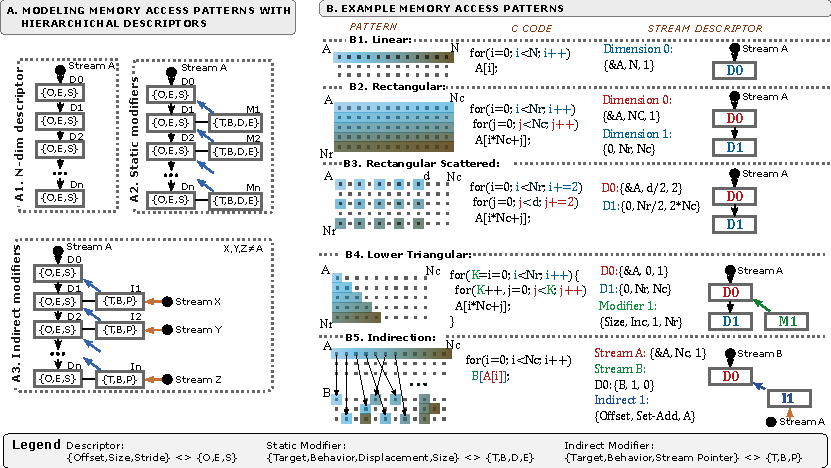
\includegraphics[width=.87\linewidth]{images/UVE-Descriptors.pdf}
 		\caption{Examples of memory access patterns with UVE descriptors - Figure adapted from \cite{uve-paper}}
 		\label{fig:stream-descriptors}
	\end{center} 
\end{figure}



\subsubsection{ISA Extension}
To support the added functionalities of the streaming data structures and the use/manipulation of SIMD vector operations, the ISA needs to be extended with the following type of instruction: 
\begin{itemize}
    \item \textbf{Stream configurations}, as the name implies, these instructions are responsible for encoding the descriptors/modifiers described above, controlling the behavior of the streaming engine. 

    \item \textbf{Stream control} instructions enable the control of streams and allow vector registers to stop/restore momentarily. This behavior control enables the execution of multiple processes without interfering with stream configurations.

    \item \textbf{Predication and masking} allow the control of execution of SIMD operations by disabling selected lanes. The proposed UVE provides instructions for predicate configuration based on comparisons and valid vector register elements.

    \item \textbf{Loop control} is assured through three conditional branch instructions: predicate-based (condition tested on a specific predicate register), end-of-stream (a condition on the end of a stream), and end-of-dimension (a condition on a stream dimension end).

    \item \textbf{Vector manipulation} instructions allow the common arithmetic, logic, and shift operations to be applied to the vector registers.
\end{itemize}


\subsubsection{Experimental Results}

All workload tests were conducted using a CPU simulation modeled after an ARM Cortex A76. The result analysis involved comparing the UVE streaming engine implementation with two ARM cores: one featuring only the ARM NEON Extension and the other supporting the ARM SVE.

The overall performance results demonstrated a significant advantage of 2.4x over the ARM SVE. The UVE's speedup was attributed to the reduction in compiled code and the streaming infrastructure, which effectively decreased load-to-use latency and enhanced memory utilization.

\section{Discussion}
The presented overview of the state-of-the-art showcases the existing potential to obtain relevant performance gains through the mutual exploitation of the data streaming and vector processing in RISC-V processor architectures. In particular, the outcomes from the presented proof-of-concept implementation of UVE with Data Streaming Support underscore the need for a thorough hardware description evaluation to validate the potential of this system.

With these considerations in mind, the focal point of this thesis shall be the implementation of the proposed Instruction Set Architecture (ISA) and streaming engine on the 6-stage, single-issue CPU, the CVA6 (as detailed in the subsequent chapter).

The development of such CPU configuration will establish the essential infrastructure for comprehensive testing and evaluation of the system. For instance, it will enable the assessment of performance against alternative hardware implementations of the CPU with streaming and vector manipulation capabilities. Additionally, having this infrastructure in place will facilitate energy consumption and design footprint analyses, allowing for insightful comparisons.





%%%%%%%%%%%%%%%%%%%%%%%%%%%%%%%%%%%%%%%%%%%%%%%%%%%%%%%%%

